
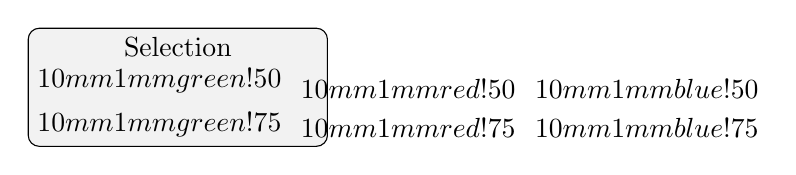
\begin{tikzpicture}
    \tikzstyle{box} = [rectangle, rounded corners, minimum width=3.8cm, minimum height=1.5cm,text centered, draw=black, fill=gray!10]

    \node [box] (selection) {};
    \node [anchor=north] at (selection.north) {Selection};

    \node (line1) [anchor=south west] at (selection.south west) {$\coloredrule{10mm}{1mm}{green!75}$};
    \node (line2) [anchor=south west] at (line1.south east) {$\coloredrule{10mm}{1mm}{red!75}$};
    \node (line3) [anchor=south west] at (line2.south east) {$\coloredrule{10mm}{1mm}{blue!75}$};
    \node (line4) [anchor=south west] at (line1.north west) {$\coloredrule{10mm}{1mm}{green!50}$};
    \node (line5) [anchor=south west] at (line2.north west) {$\coloredrule{10mm}{1mm}{red!50}$};
    \node (line6) [anchor=south west] at (line3.north west) {$\coloredrule{10mm}{1mm}{blue!50}$};

  \end{tikzpicture}